\section{Свойства гармонических функций в $\R^3$: бесконечная дифференцируемость, теорема о среднем. Обратная теорема о среднем.}
% Затехала Ермолова Марина
\begin{definition} Функция $u(x)$ гармоническая в $\Omega \in \R^3$, если 
\begin{enumerate}
\item $u(x) \in C^2 (\Omega)$
\item $\Delta u(x) = 0 \Forall x \in \Omega$ 
\end{enumerate}
\end{definition}
\begin{theorem}
Всякая функция $u(x)$, гармоническая в области $\Omega$, является в $\Omega$ бесконечно дифференцируемой, т.е. $u(x) \in C^{\infty}(\Omega).$
\end{theorem}
\begin{proof}
Возьмем $x_0 \in \Omega$ и $\overline{B}_r(x_0) \subset \Omega$. Представим $u(x)$ суммой: $$u(x)= - \oint\limits_{|y-x_0|=r} \bigg( \frac{-1}{4\pi |x-y|} \bigg) \frac{\partial u(y)}{\partial \vec{n_y}} dS_y + \oint\limits_{|y-x_0|=r} u(y) \frac{\partial}{\partial \vec{n_y}} \bigg(\frac{-1}{4\pi |x-y|}\bigg) dS_y $$
\begin{center}
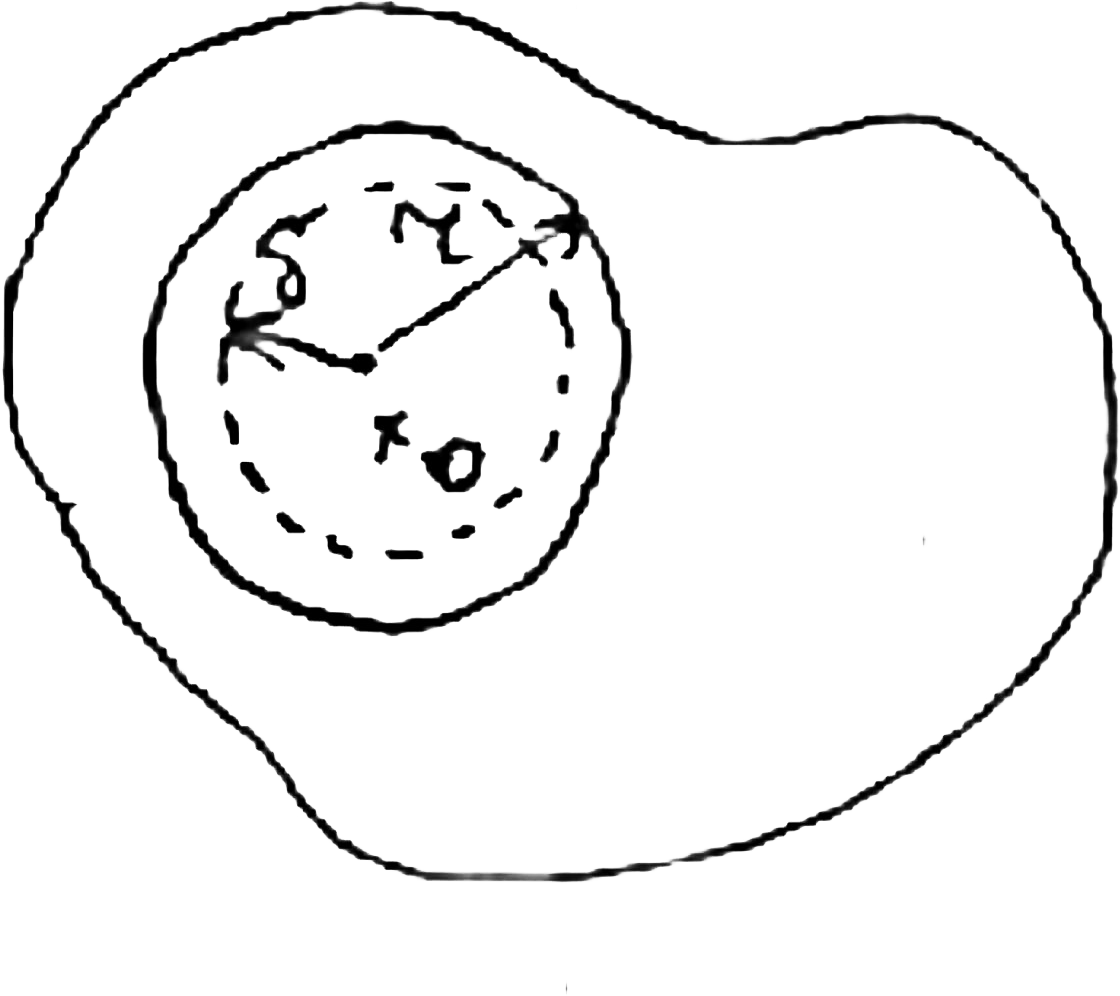
\includegraphics[width=0.2\textwidth]{17_2_new}
\end{center}
Теперь берем $B_{\delta}(x_0) \subsetneq B_{r}(x_0).$ Будем обозначать $S(x_0,r)$ сферу $\partial B_r(x_0).$ Если $x \in \overline{B}_{\delta}(x_0), y \in S(x_0,r)$, то $|x-y| \geq r - \delta > 0.$\\
Рассмотрим в $\overline{B}_{\delta}(x_0)$ $$u_0(x)= \oint\limits_{|y-x_0|=r} \bigg( \frac{-1}{4\pi |x-y|} \bigg) \frac{\partial u(y)}{\partial \vec{n_y}} dS_y.$$
Напишем $$\tilde{u_0}(x) = \oint\limits_{|y-x_0|=r} D_x^\alpha \bigg( \frac{-1}{4\pi |x-y|} \bigg) \frac{\partial u(y)}{\partial \vec{n_y}} dS_y$$
Заметим, что $\frac{-1}{4\pi |x-y|} \in C^{\infty}( \overline{B}_{\delta}(x_0) \times S(x_0,r)) \Rightarrow$ записанные частные производные непрерывны, интеграл $\tilde{u_0}$ существует $\Rightarrow \tilde{u_0}(x) = D_x^\alpha u_o(x).$\\
Теперь берем $$u_2(x) = \oint\limits_{|y-x_0|=r} u(y) \frac{\partial}{\partial \vec{n_y}} \bigg(\frac{-1}{4\pi |x-y|}\bigg) dS_y$$ 
$$\frac{\partial}{\partial \vec{n_y}} \bigg(\frac{-1}{4\pi |x-y|}\bigg) = \sum_1^n n_k \frac{\partial}{\partial \vec{y_k}} \bigg(\frac{-1}{4\pi |x-y|}\bigg)$$ В $\overline{B}_{\delta}(x_0)$ запишем 
$$\tilde{u_2}(x)=\sum_1^3 \oint u_0(y) n_k (y) D_x^\alpha \bigg(\frac{\partial}{\partial \vec{y_k}} \bigg(\frac{-1}{4\pi |x-y|}\bigg)dS_y$$
Записанные частные производные непрерывны, интеграл $\tilde{u_2}(x)$ существует $\Rightarrow \tilde{u_2}(x)=D_x^\alpha u_2(x).$\\
Итак, для $u_0(x)$ и $u_2(x)$ существуют частные производные любого порядка. Значит, $u(x) \in  C^{\infty}( \overline{B}_{\delta}(x_0)),$ где\\ $x_0$ - произвольная точка из $\Omega. \Rightarrow u(x) \in C^{\infty}(\Omega)$
\end{proof}
\begin{theorem}[Теорема о среднем]
Пусть $u(x)$, гармоническая в шаре $B_r(x_0)$ и $u(x) \in C^1(\overline{B}_r(x_0))$. Тогда $u(x_0)= \frac{1}{4\pi r^2} \int \limits_{|y-x_0|=r}u(y)dS_y.$ (в центре - среднее по значениям на сфере)
\end{theorem}
\begin{proof}
$$u(x_0)= -\oint\limits_{|y-x_0|=r} \bigg( \frac{-1}{4\pi |x_0-y|} \bigg) \frac{\partial u}{\partial \vec{n_y}} dS_y + \oint\limits_{|y-x_0|=r} u(y) \frac{\partial}{\partial \vec{n_y}} \bigg(\frac{-1}{4\pi |x_0-y|}\bigg) dS_y $$
$$\frac{\partial}{\partial \vec{n_y}} \bigg(\frac{-1}{4\pi |x_0-y|}\bigg)\stackrel{\rho = |x_0 - y|}{=} \frac{-1}{4\pi}\frac{\partial}{\partial \rho}\frac{1}{\rho} = \frac{1}{4 \pi r^2},$$ тогда $$\oint\limits_{|y-x_0|=r} u(y) \frac{\partial}{\partial \vec{n_y}} \bigg(\frac{-1}{4\pi |x_0-y|}\bigg) dS_y = \frac{1}{4 \pi r^2} \oint\limits_{|y-x_0|=r} u(y) dS_y.$$
Покажем, что потенциал простого слоя равен нулю.
\[ -\oint\limits_{|y-x_0|=r} \bigg( \frac{-1}{4\pi |x_0-y|} \bigg) \frac{\partial u(y)}{\partial \vec{n_y}} dS_y = \frac{1}{4\pi} \frac{1}{r} \oint\limits_{|y-x_0|=r}  \frac{\partial u(y)}{\partial \vec{n_y}} dS_y = \frac{1}{4\pi r} \oint\limits_{|y-x_0|=r} (\nabla u(y), \vec{n}(y)) dS_y \stackrel{\text{ф-ла Остр.-Гаусса}}{=}
\]
\[
 = \frac{1}{4\pi r} \oint\limits_{|y-x_0|<r} \div(\nabla u) dy = \frac{1}{4\pi r} \oint\limits_{|y-x_0|<r} \Delta u dy  = 0
 \]
\end{proof}
\begin{theorem}[Обратная теорема о среднем]
Пусть $u(x) \in C(\Omega)$ и $u(x)$ обладает свойством среднего $\forall x \in \Omega$, где $\Omega \in \R^3$ - произвольная область. Тогда $u(x)$ - гармоническая функция на $\Omega$. 
\end{theorem}
\begin{proof}
$\forall x_0\in\Omega\Exists r > 0: \overline{B(x_0, r)}\subset\Omega.$ 
Рассмотрим решение $$v(x) = \frac{1}{4\pi R}\oint\limits_{|y|=r}\frac{r^2-|x|^2}{|y-x|^3}u(y)dS_y $$ 
$$\text{для задачи} \begin{cases}
\Delta u(x) = 0, |x| < r \\
\while{v}{|x| = r} = \while{u}{|x| = r}
\end{cases} $$
Введем $w(x) = u(x) - v(x)$, $w(x) \in C(|x| \leq r)$, получим что $w(x)$ удовлетворяет свойству среднего. Тогда по принципу максимума (для функции, удовлетворяющей свойству среднего, будет доказан в следующем билете) $|w(x)| \leq \max\limits_{|y-x| = r}|w(y)| = 0  \Rightarrow u(x) = v(x) \Forall x\colon |x| < r$
\end{proof}